\documentclass[a4paper,10pt]{book}

\usepackage[latin1]{inputenc}
\usepackage[italian]{babel}
\usepackage[pdftex]{graphicx}

\title{Reti Neurali}
\author{Davide Gessa}
\date{14-04-2010}

\pdfinfo{%
  /Title    (Reti Neurali)
  /Author   (Davide Gessa)
  /Subject  ()
  /Keywords (reti neurali fuzzy statistica matematica)
}

\begin{document}
\maketitle

\tableofcontents
\setcounter{tocdepth}{4}
\listoffigures
\listoftables


\chapter{Introduzione}
Questa tesi nasce da un vecchio software da me iniziato verso l'inizio del 2009 (e
mai terminato) che riassumeva il frutto di qualche mia curiosita' riguardo 
l'argomento delle reti neurali artificiali; qualche mese fa ho ritrovato i sorgenti e mi son 
reinteressato all'argomento, riscrivendo da zero un nuovo software (che analizzero' 
in seguito) che implementa alcuni tipi di reti neurali artificiali e loro applicazioni
pratiche. Avenvo gia' iniziato una breve trattazione da esporre su un altro mio
progetto, ma ho deciso di iniziare da capo per dedicarmi ad un argomento che
raccoglie in se' piu' materie.

\section{Licenza}
Il proggetto e' rilasciato interamente sotto licenza GPLv2, e' riportato qui di 
seguito l'header presente in ogni file sorgente del progetto:
\newline
\newline 
\ttfamily
\textit
    libneuralnetwork
    Copyright (C) 2010 Davide Gessa
    
    This program is free software: you can redistribute it and/or modify
    it under the terms of the GNU General Public License as published by
    the Free Software Foundation, either version 2 of the License, or
    (at your option) any later version.

    This program is distributed in the hope that it will be useful,
    but WITHOUT ANY WARRANTY; without even the implied warranty of
    MERCHANTABILITY or FITNESS FOR A PARTICULAR PURPOSE.  See the
    GNU General Public License for more details.

    You should have received a copy of the GNU General Public License
    along with this program.  If not, see <http://www.gnu.org/licenses/>.
\rmfamily
\newline


\section{Strumenti software}
Ecco una lista dei software principali utilizzati per realizzare il progetto e la tesi
che state leggendo; da sottolineare che tutti sono free software e opensource, e che 
lo sviluppo e' avvenuto coi sistemi gnu/linux gentoo, gnu/freebsd gentoo, anch'essi free
e opensource.

\begin{description}
\item[gcc] compilatore per il linguaggio C
\item[cmake] sistema di compilazione
\item[geany] C ide
\item[winefish] latex ide 
\item[subversion] controllo di revisione
\item[latex] compilatore per il linguaggio \LaTeX
\end{description}



\section{\LaTeX}
Per scrivere la documentazione del sistema e' stato utilizzato il linguaggio di markup
\LaTeX, che permette di preparare dei testi basati su \TeX, un linguaggio di composizione 
tipografica. Utilizzare \LaTeX, permette di risparmiare un tempo notevole per quanto riguarda
la formattazione delle pagine, la creazione degli indici, la visualizzazione di formule matematiche
e molto altro, e per questo motivo e' utilizzato da gran parte di accademici, scienziati, matematici
e ingegneri. \LaTeX e' distribuito come software libero ed e' disponibile su molte piattaforme.





\chapter{Reti neurali}
\section{In natura}
Il funzionamento delle reti neurali artificiali, deriva dalle reti neurali presenti
in natura nel cervello degli animali; i primi successi significativi riguardo lo studio 
del funzionamento delle reti neurali sono relativamente recenti, e alcuni aspetti
del loro funzionamento sono ancora ignoti.
Le reti neurali sono delle strutture costituite da neuroni; 
I neuroni sono classificabili in base alla loro funzione in:
 - Neuroni sensitivi o neuroni di input: si occupano di ricevere impulsi e stimoli 
	dagli organi sensoriali.
 - Neuroni motori o neuroni di output: generano impulsi di tipo motori che vengono
	trasmessi agli organi periferici.
 - Interneuroni o neuroni nascosti: elaborano le informazioni fornite dai neuroni 
	sensitivi per trasmetterle ai neuroni motori.
 
Un neurone e' formato da:

 - La soma: che comprende il nucleo e altri apparati dedicati alla sopravvivenza della
	cellula.
 
 - Gli assoni: conducono il segnale generato dal soma verso altre cellule neuronali.
 
 - I dentriti: son costituiti da diramazioni ad albero che trasportano segnali di altri
	neuroni, verso la soma; i dentriti hanno la caratteristica di non essere buoni
	conduttori di segnali nervosi, i segnali ricevuti tendono quindi a diminuire di
	intensita'.

% Da cambiare, e' proprieta' del governo federale O_O
\begin{figure}[h]
	\begin{center}	
		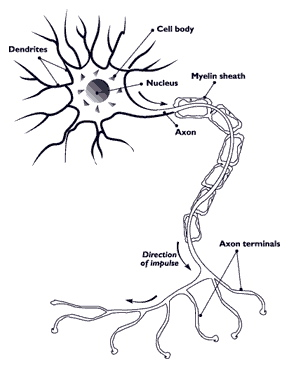
\includegraphics[scale=0.50]{img/neuron.jpg}
		\caption{Struttura di un neurone}
		\label{fig: Struttura di un neurone}
	\end{center}
\end{figure}
 
\subsection{Trasmissione degli impulsi tra neuroni}
% Parla delle sinapsi, delle connessioni e dei pesi



\section{Reti neurali artificiali}
Le reti neurali artificiali, imitano in parte il funzionamento delle
reti neurali naturali;

\subsection{Storia}

\subsection{Tipi di rete}



\chapter{Pattern Recognition}




%\begin{table}[h]
%	\begin{center}
%	    \begin{tabular}{ | c | c | }
%	    \hline
%	    Caratteristica & Quantita' \\ \hline
%	    File aperti & 32.000  \\ \hline
%	    FS montati in contemporanea & 0 \\ \hline
%	    Task in esecuzione & 0   \\ \hline
%	    Numero massimo allocazioni & 4096 \\ \hline
%	    Driver caricati & 0  \\ \hline	    
%	    \end{tabular}
%	\end{center}
%	\caption{Prestazioni generiche}
%	\label{tab:generic_benchmarks}
%\end{table}




\chapter{Bibliografia}
\begin{thebibliography}{Bibliografia}
	\bibitem{lamport-latex2} 
	\bibitem{lamport-latex2} 
	\bibitem{lamport-latex2} 
	\bibitem{lamport-latex2} 
\end{thebibliography}

\appendix


\end{document}

